% !TeX root = ../main.tex
% Add the above to each chapter to make compiling the PDF easier in some editors.

\chapter{Bewertungsdiagramme}\label{chapter:Bewertungsdiagramme}

\begin{savenotes}
	\begin{figure}[H]
		\centering
		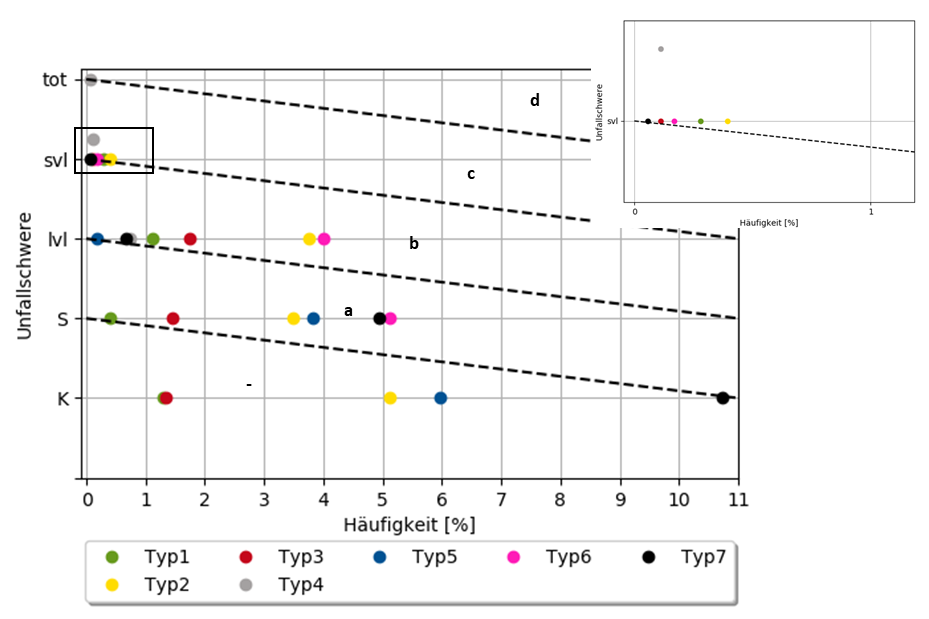
\includegraphics[width=12cm,height=8cm]{figures/Bewertung_UTF(2)}
		\caption[Bewertung der Unfälle im Testgebiet anhand der sieben Unfalltypen ohne Typ 6 bei den Kleinunfällen]{Bewertung der Unfälle im Testgebiet anhand der sieben Unfalltypen ohne Typ 6 bei den Kleinunfällen}\label{fig:Bewertung_UTF(2)}
	\end{figure}
\end{savenotes}

\begin{savenotes}
	\begin{figure}[H]
		\centering
		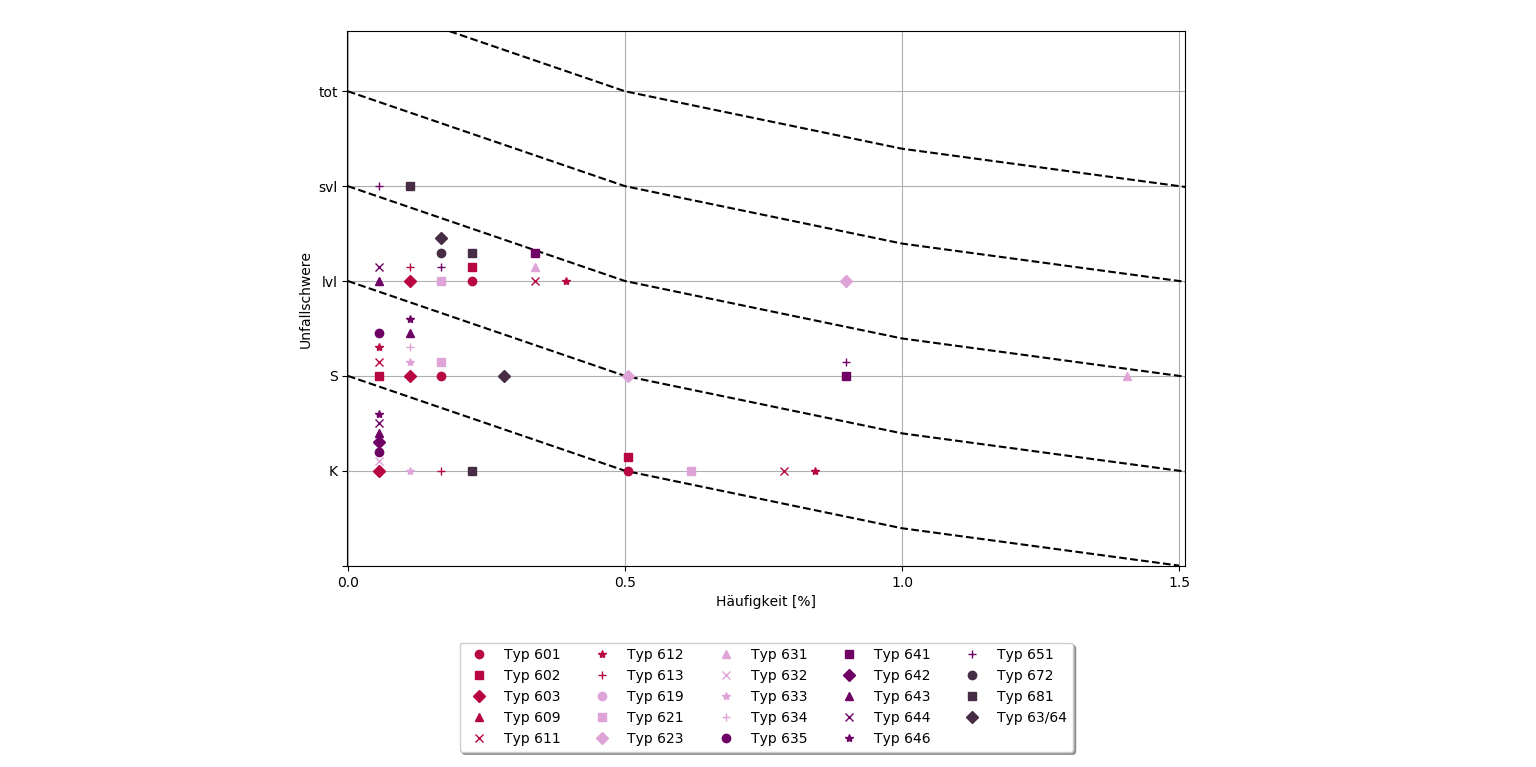
\includegraphics[width=12cm,height=8cm]{figures/Bewertung_FT6(2)}
		\caption[Ausschnitt aus der Bewertung der Unfälle, denen ein Feintyp des Unfalltyps 6 zugeordnet wurde]{Ausschnitt aus der Bewertung der Unfälle, denen ein Feintyp des Unfalltyps 6 zugeordnet wurde}\label{fig:Bewertung_FT6(2)}
	\end{figure}
\end{savenotes}


\begin{savenotes}
	\begin{figure}[H]
		\centering
		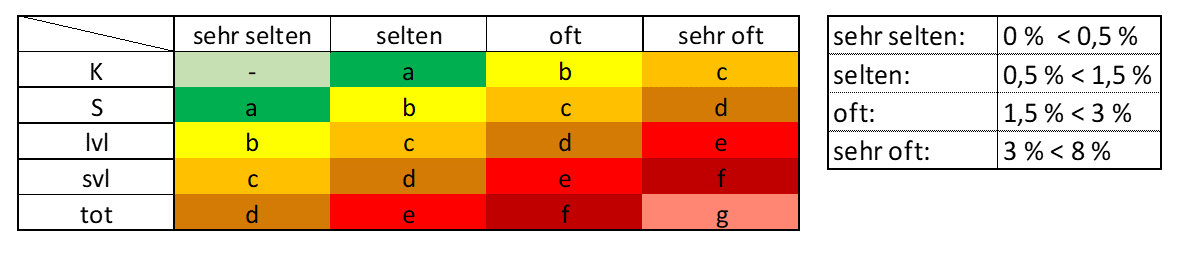
\includegraphics[width=16cm,height=4cm]{figures/Eintrittswahrscheinlichkeit}
		\caption[Bestimmung der Risiko Kategorie anhand der Eintrittswahrscheinlichkeit und Unfallschwer]{Bestimmung der Risiko Kategorie anhand der Eintrittswahrscheinlichkeit und Unfallschwere}\label{fig:Eintrittswahrscheinlichkeit}
	\end{figure}
\end{savenotes}

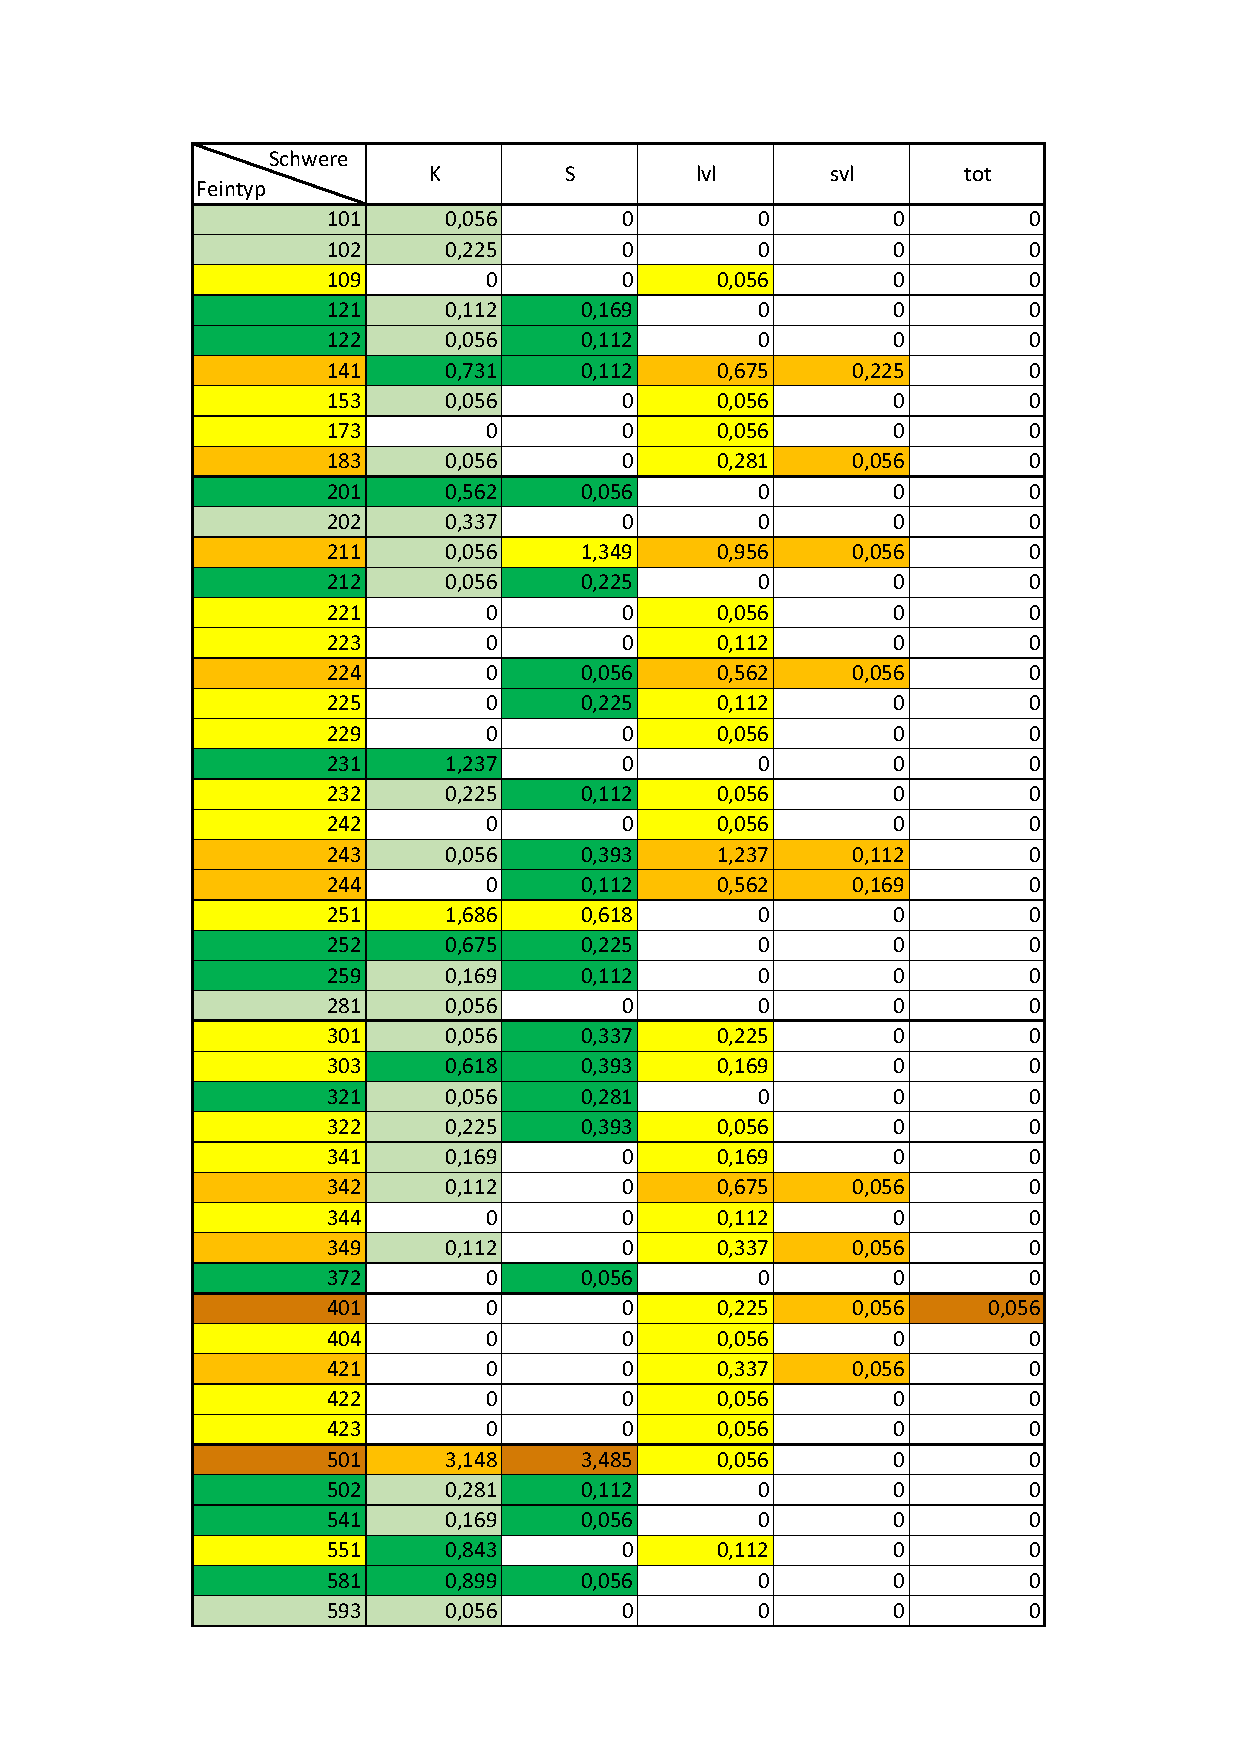
\includepdf[pages={1-2}, pagecommand={\thispagestyle{fancy}}, width=\textwidth, height=\textheight, frame=false]{figures/Feintypen.pdf}

%Pdf der Exceltabelle mit den Häufigkeiten einfügen, kurz dazu schreiben, dass diese Häufigkieten in den Grafiken dargestellt wurden. Evtl. an den Anfang des Anhang-Kapitels stellen.